\documentclass[hyperref={unicode}]{beamer}
\mode<presentation> {
\usetheme{Warsaw}
\setbeamercovered{transparent}
}
\usecolortheme{rose}
\usepackage[czech]{babel}
\usepackage[utf8]{inputenc}
\usepackage{amsmath, amsthm, amssymb}
\usepackage{times}
\usepackage{graphics}


\title{Typografie a~publikování\,--\,5.~projekt}
\subtitle{Konečné automaty}
\author{Alex Sporni\texorpdfstring{\\ xsporn01@stud.fit.vutbr.cz}{}}
\date{\today}
\institute
{
	Vysoké učení technické v~Brně\\
	Fakulta informačních technologií
}

\begin{document}
%#1
\begin{frame}
\titlepage
\end{frame}
%#2
\begin{frame}
\transblindshorizontal
\frametitle{Konečné automaty}
\textbf{Definice a~základní principy konečných automatů a jejich uplatnění:}\\
Konečný automat je teoretický výpočetní model používaný v~informatice pro studium formálních jazyků. Popisuje velice jednoduchý počítač, který může být v~jednom z~několika stavů, mezi kterými přechází na základě symbolů, které čte ze vstupu.
\begin{itemize}
\pause
\item{Konečný automat (KA) budeme chápat jako abstraktní model určitého specifického typu výpočtu.}
\pause
\item{Výpočet neprobíhá s~čísly, ale s~objekty, které budeme nazývat symboly}
\pause
\item{Tento model má v~informatice a~výpočetní technice široké použití, jako např.:}
\pause
\begin{itemize}
\item{při návrhu sekvenčních logických obvodů}
\item{v~překladačích programovacích jazyků}
\item{při řešení jednodušších úloh z~oblasti umělé inteligence}
\item{v~řídicích systémech logického typu}
\end{itemize}
\end{itemize}
\end{frame}
%#3
\begin{frame}
\transblindshorizontal
\frametitle{Typy KA}
Podíváme-li se na KA jako na „černou skříňku“ (zajímá nás tedy pouze to, jak automat komunikuje s~okolím, tj. jak z~okolí přijímá informaci a jakou informaci do okolí vydává; naopak nás vůbec nezajímá „co se děje uvnitř“), lze rozlišovat tři typy KA:
\begin{enumerate}
\item{rozpoznávací KA (akceptor)}
\item{klasifikační KA (klasifikátor)}
\item{KA s~výstupní funkcí (translátor)}
\end{enumerate}
\end{frame}
%#4
\begin{frame}
\transblindshorizontal
\frametitle{Typy KA\,--\,Rozpoznávací automat}
\begin{block}{Definice}
\begin{itemize}
\item{Rozpoznávací automat o~zpracovaném řetězci vydá jednoznačné rozhodnutí typu ano/ne}
\item{symbolicky můžeme toto rozhodnutí znázornit jako žárovku na výstupu, která buď svítí, nebo nesvítí}
\end{itemize}
\end{block}
\begin{figure}[h]
		\centering
		\scalebox{0.4}{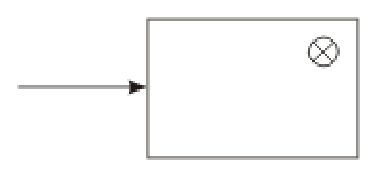
\includegraphics{autom1.eps}}
\end{figure}
\end{frame}
%#5
\begin{frame}
\transblindshorizontal
\frametitle{Typy KA\,--\,Klasifikační KA}
\begin{block}{Definice}
\begin{itemize}
\item{Klasifikační automat zpracovaný řetězec zařadí do jedné z~\textit{n} tříd}
\item{Symbolicky můžeme toto rozhodnutí znázornit jako \textit{n} žárovek, z~nichž v~každém okamžiku svítí právě jedna}
\end{itemize}
\end{block}
\begin{figure}[h]
		\centering
		\scalebox{0.4}{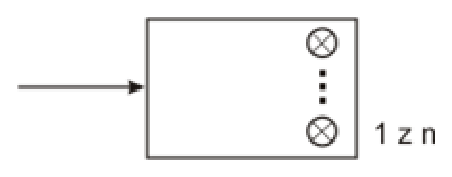
\includegraphics{autom2.eps}}
\end{figure}
\end{frame}
%#6
\begin{frame}
\transblindshorizontal
\frametitle{Typy KA\,--\,Automat s~výstupní funkcí }
\begin{block}{Definice}
\begin{itemize}
\item{Automat s~výstupní funkcí na základě vstupního řetězce vytvoří \textit{výstupní řetězec} ze symbolů \textit{z~množiny výstupních symbolů.}}
\item{To, že automat generuje výstupní řetězce, je v~symbolickém obrázku znázorněno výstupní šipkou}
\end{itemize}
\end{block}
\begin{figure}[h]
		\centering
		\scalebox{0.4}{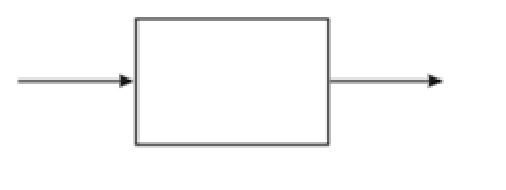
\includegraphics{autom3.eps}}
\end{figure}
\end{frame}
%#7
\begin{frame}
\transblindshorizontal
\frametitle{Formální definice}
Formálně je konečný automat definován jako uspořádaná pětice ($S, \Sigma, \sigma, s, A$)
\begin{itemize}
\item{$S$ je konečná neprázdná množina stavů}
\item{$\Sigma$ je konečná neprázdná množina vstupních symbolů}
\item{$\sigma$ je tzv. přechodová funkce (též přechodová tabulka), popisující pravidla přechodů mezi stavy. Může mít buď podobu $S \times \Sigma \rightarrow S$ (deterministický automat), nebo $S \times {\Sigma \cup \epsilon} \rightarrow P(S)$ (nedeterministický automat)}
\item{$s$ je počáteční stav, $s \in S$}
\item{$A$ je množina přijímajících stavů, $A \subseteq S$ }
\end{itemize}
\end{frame}
%#8
\begin{frame}
\transblindshorizontal
\frametitle{Způsoby reprezentace konečných automatů}
\begin{block}{}
Matematický popis KA pomocí definice uvedený v~předchozím textu je sice jednoznačný a úplný, nicméně pro praktické použití bývají výhodnější jiné způsoby popisu automatu:
\begin{itemize}
\item{přechodový graf (stavový diagram)\,--\,grafická reprezentace, pro výukové účely nejvhodnější}
\item{tabulka\,--\,tabulková reprezentace, méně názorná, vhodné východisko pro implementaci}
\item{stavový strom\,--\,kompromis mezi oběma předchozími způsoby}
\end{itemize}
\end{block}
\end{frame}
%#9
\begin{frame}
\transblindshorizontal
\frametitle{Reprezentace KA\,--\,stavovým diagramem}
\begin{alertblock}{}
\begin{itemize}
\item{stavům KA odpovídají vrcholy grafu (kolečka)}
\item{přechodům orientované hrany mezi nimi}
\item{hrany jsou ohodnoceny vstupními symboly představují podněty k~provedení přechodu}
\item{počáteční stav je označen vstupní šipkou}
\item{koncové stavy jsou označeny výstupními šipkami}
\end{itemize}
\end{alertblock}
\begin{figure}[h]
		\centering
		\scalebox{0.35}{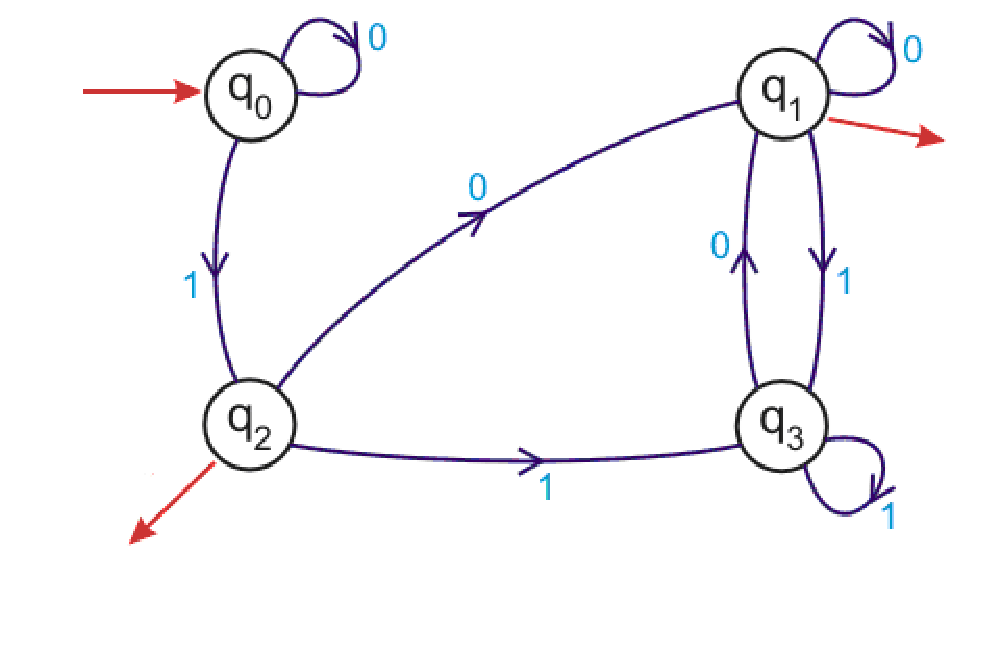
\includegraphics{autom4.eps}}
\end{figure}
\end{frame}
%#10
\begin{frame}
\transblindshorizontal
\frametitle{Reprezentace KA\,--\,tabulkou}
\begin{alertblock}{}
\begin{itemize}
\pause
\item{stavům odpovídají řádky tabulky}
\pause
\item{vstupním symbolům její sloupce}
\pause
\item{každé políčko tabulky tedy odpovídá právě jedné dvojici (stav, vstupní symbol)}
\pause
\item{v~odpovídajících pozicích jsou zapsány následující stavy příslušných přechodů}
\pause
\item{rádek odpovídající počátečnímu stavu je označen vstupní šipkou}
\pause
\item{řádky odpovídající koncovým stavům jsou označeny výstupními šipkami}
\pause
\end{itemize}
\end{alertblock}
\begin{figure}[h]
		\centering
		\scalebox{0.40}{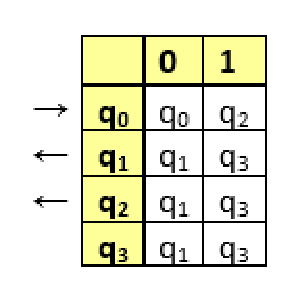
\includegraphics{autom5.eps}}
\end{figure}
\end{frame}
%#11
\begin{frame}
\transblindshorizontal
\frametitle{Reprezentace KA\,--\,stavovým stromem}
\begin{alertblock}{}
\begin{itemize}
\item{Strom začínáme vytvářet od počátečního stavu}
\item{Postupně budeme přidávat pro každý vstupní symbol jednu hranu orientovanou směrem dolů}
\item{Rozvoj stromu pokračuje tak dlouho, dokud se v~listech stromu neobjeví stavy, jejichž výskyty jsou již někde ve stromu rozvinuty}
\item{Počáteční stav není třeba nijak označovat, je zřejmý z~toho, že je kořenem stromu}
\item{Výstupní stavy jsou označeny výstupními šipkami u~všech jejich výskytů}
\end{itemize}
\end{alertblock}
\begin{figure}[h]
		\centering
		\scalebox{0.30}{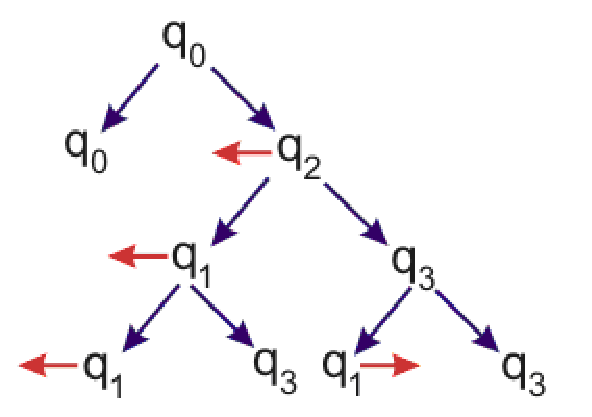
\includegraphics{autom6.eps}}
\end{figure}
\end{frame}
%#12
\begin{frame}
\transblindshorizontal
\frametitle{{Použité zdroje}}
\begin{itemize}
\item{Václav Vais\,--\,Konečné automaty: \url{https://bit.ly/2qN3Q2S}}
\item{Wikipedia:\\ \url{https://bit.ly/2HGBGBn}}
\end{itemize}	
\end{frame}

\end{document}

